\documentclass{beamer}
\beamertemplatenavigationsymbolsempty
\usecolortheme{beaver}
\setbeamertemplate{blocks}[rounded=true, shadow=true]
\setbeamertemplate{footline}[page number]
%
\usepackage[utf8]{inputenc}
\usepackage[english,russian]{babel}
\usepackage{amssymb,amsfonts,amsmath,mathtext}
\usepackage{subfig}
\usepackage[all]{xy} % xy package for diagrams
\usepackage{array}
\usepackage{multicol} % many columns in slide
\usepackage{hyperref} % urls
\usepackage{hhline} %tables
\usepackage{comment} %comments
% Your figures are here:
\graphicspath{ {fig/} {../fig/} }
\usepackage{sepfootnotes}
\DeclareMathOperator\supp{supp}
\usepackage{tikz}

%----------------------------------------------------------------------------------------------------------

\title[\hbox to 56mm{Многократное обучение}]{Вырождение распределений при  многократном  \\ обучении в рекомендательных системах}
\author[Н.\,А.~Крехов]{Николай Александрович Крехов}
\institute{Московский физико-технический институт}
\date{\footnotesize
\par\smallskip\emph{Курс:} Моя первая научная статья
\par\smallskip\emph{Эксперт:} к.ф.-м.н. А.\,С.~Хританков
\par\smallskip\emph{Консультант:} А.\,С.~Веприков
\par\bigskip\small 2024}

%----------------------------------------------------------------------------------------------------------

\begin{document}

%----------------------------------------------------------------------------------------------------------

\begin{frame}

    \thispagestyle{empty}
    \maketitle
    
\end{frame}

%-----------------------------------------------------------------------------------------------------

\begin{frame}{Цель исследования}
    \begin{block}{Цель}
        Исследование вырождения распределений пользователей и товаров в динамической системе с рекомендательным алгоритмом.
    \end{block}
    \begin{block}{Задача}
        Предложить алгоритм, который улучшает стандартные метрики для рекомендательных алгоримтов при условии, что в пределе не возникает вырождения распределения товаров и пользователей.
    \end{block}

\end{frame}

%-----------------------------------------------------------------------------------------------------

\begin{frame}{Алгоритм рекомендации}

\item  \footnotesize Функция $u_{\text{true}}(c, w, z)$ отражает интерес пользователя $c$ к товару

\item  \footnotesize Сделка: $y_{c,w} \sim Bern(u_{\text{true}}(c, w, z))$

\item Рассматриваем класс рекомендательных алгоритмов, которые оценивают $u_{\text{true}}(c, w, z)$ через $u_{\text{pred}}(c, w)$

\begin{columns}[c]

    \column{0.55\textwidth}
    Рекомендательный алгоритм:
        \begin{enumerate}
            \item Вычисляет функцию $u_{\text{pred}}(c, w)$ для всех $c,\ w$
            \item Для каждого $c$ по функци $u_{\text{pred}}$ выбирает множество товаров размера $k$ для рекомендации: $\{w_{i_1},\ldots, w_{i_k}\}$
        \end{enumerate}
    
    \column{0.60\textwidth}
        \begin{tikzpicture}
            \node[draw, rectangle] (customer) at (0,0) {Customer $(c^{d_1},\ldots,c^{d_c})^T$};
            \node[draw, circle, text width=2cm] (item1) at (-2,-3) {Item 1  $(w_1^{d_1},\ldots,w_1^{d_w})^T$};
            \node[draw, circle, text width=2cm] (item2) at (2,-3) {Item 2 $(w_2^{d_1},\ldots,w_2^{d_w})^T$};
            
            \draw[->, green] (customer.200) to[out=-135,in=90] node[midway, above, sloped] {\scriptsize $y_{c, w^1} = 1$} (item1);
            \draw[->] (item1.45) to[out=45,in=-45] (customer.200);
    
            
            \draw[->, red] (customer.-20) to[out=-135,in=135] node[midway, above, sloped] {\scriptsize$y_{c, w^2} = 0$} (item2);
            \draw[->] (item2.90) to[out=45,in=-45] (customer.-20);
    
        \end{tikzpicture}

\end{columns}
Примеры алгоритмов:

    \begin{itemize}
        \item[-] TopPopularity
        \item[-] Random
        \item[-] Collaborative Filtering using SVD
    \end{itemize}    
    
\end{frame}

%-----------------------------------------------------------------------------------------------------


\begin{frame}{Математическая постановка задачи}
 \scriptsize{Пользователи  и товары: $C \subset \mathbb{R}^d, W \subset \mathbb{R}^l$. На каждом шаге $t$ имеется совместное распределение: $(c, w)^T \sim p^{t}_{c,w} (x_c , x_w )$ \\
 $u^t_{\text{true}}: \mathbb{R}^{d_c} \times \mathbb{R}^{d_w} \times \Omega_z \to [0; 1]$ - функция полезности товара для данного пользователя.}
 \\
 $u^t_{\text{pred}}: \mathbb{R}^{d_c} \times \mathbb{R}^{d_w} \to [0; 1]$ - оценивающая $u^t_{\text{true}}$ функция.
\\$D_t$ - оператор эволюции распределения:
$p^{t + 1}(x_c, x_w) = \text{D}_t(p^{t})(x_c, x_w)$

Будем говорить, что распределение $p^t(x)$ вырождается, если 
$$
\mu (\supp p^{\infty}(x)) = 0,
$$ где $p^{\infty} = \lim_{t\to \infty} {p^t(x)}
$

    \begin{columns}[c]
    
        \column{0.6\textwidth}
            \begin{figure}
                    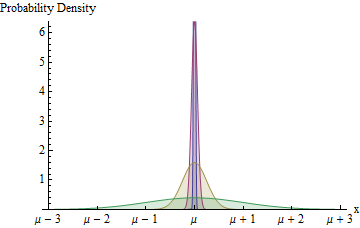
\includegraphics[width=0.9\textwidth]{images/degenerating.png}
            \end{figure}
            
        \column{0.6\textwidth}
            Введем функционал
            $$L^t(c, w) = \mathbb{E}_z[(u_{\text{true}}(c, w, z) - u_{\text{pred}}(c, w))^2],$$
            Согласно ему, начиная с некоторого $t=\tau$ и будет изменяться распределение:
            $$
            p^{t+1}_{c, w}  \propto L^t(c, w)^{-1}
            $$
            
        
            
    \end{columns}

\end{frame}

%-----------------------------------------------------------------------------------------------------

\begin{frame}{Публикации по теме}
    \begin{itemize}
    
    \item $[1]$ A. S. Vepricov, A. S. Khritankov. On the problem of repeated supervised learning \url{https://github.com/intsystems/2023-Project-119/blob/master/paper/M1P.pdf}.

    \item $[2]$ Anton Khritankov. Positive feedback loops lead to concept drift in machine learning systems.


    \item $[3]$ Jiang, Ray & Chiappa, Silvia & Lattimore, Tor & György, András & Kohli, Pushmeet. (2019). Degenerate Feedback Loops in Recommender Systems
  
    \end{itemize}
\end{frame}

%-----------------------------------------------------------------------------------------------------


\begin{frame}{Критерии качества модели}

Необходимым условием является невырождение распределения $p^t_{c,w}$ пользователей-товаров.

\begin{itemize}
    \item Вырождение распределения невязок: $u_{\text{true}} - u_{\text{pred}} \sim \delta(x)$, где $\delta(x)$ - дельта-функция Дирака.\\
    Условия такого вырождения описаны в статье [1], однако никаких гарантий на отсутствие выраждения $p^t_{c,w}$ нет.
    
    \item $y_{\text{true}} := Bern(u_{\text{true}})$, 
    $y_{\text{pred}} := Bern(u_{\text{pred}})$\\
    Для каждого пользователя считаем $accuracy@K = \frac{\sum^K_{k = 1} (\mathbf{I}\{y^k_{\text{pred}} = y^k_{\text{true}}\})} {K}$ и затем усредняем по всем пользователям.
    
    
\end{itemize}


\end{frame}

%----------------------------------------------------------------------------------------------------------

\begin{frame}{Основные результаты}

\scriptsize
Предположение:
Пользователи и площадка с товарами ведут себя рационально, т.е. $p^{t+1}_{c, w}  \propto L^t(c, w)^{-1}$.

$L^t(c, w) = \mathbb{E}_z[(u_{\text{true}}(c, w, z) - u_{\text{pred}}(c, w))^2]$\\
% Переписывается в виде:
% $L^t(c, w) = \mathbb{D}_z[(u_{\text{true}}(c, w, z)] + \left(\mathbb{E}_z[(u_{\text{true}}(c, w, z)] - u_{\text{pred}}(c, w)\right)^2$
Обозначим за $\Phi^t$ - множество вырождения для $p^t_{c, w}$

\begin{enumerate}
    \item $u_{\text{pred}}(c, w) = \mathbb{E}_z[(u_{\text{true}}(c, w, z)]$, тогда $L^t(c, w) = \mathbb{D}_z[(u_{\text{true}}(c, w, z)]$\\
    $\Phi^t = \left\{ (x_c, x_w)^T \in \mathbb{R}^{d_c + d_w} \; | \; \mathbb{D}_z[(u_{\text{true}}(c, w, z)]=0 \; \right\}$\\
    $\Phi^t$ - <<большое>> , поэтому вырождение пользователей-товаров может быть.
    Предполагается вырождение по <<невязкам>>.
    
    \item
    $u_{\text{pred}}(c, w)$ = 
    \begin{cases}
       1, &\text{$\mathbb{E}_z[(u_{\text{true}}(c, w, z)] \geq \frac{1}{2} $}\\
       0, &\text{иначе}
    \end{cases} \\
    $L^t(c, w) = \mathbb{D}_z[(u_{\text{true}}(c, w, z)] + \min \left(\mathbb{E}_z[(u_{\text{true}}(c, w, z)]^2; 1 -  \mathbb{E}_z[(u_{\text{true}}(c, w, z)]^2 \right)$\\
 
        $\Phi^t = \left\{ (x_c, x_w)^T \in \mathbb{R}^{d_c + d_w} \; | \; \text{для п.в. $x_z \in \Omega_z$ $u_{\text{true}}(c, w, z) = 1$ или 0 } \; \right\}$ \\
        $\Phi^t$ - <<маленькое>>, поэтому вырождения пользователей-товаров скорее всего не будет.

        \textbf{Лемма}: при таком $u_{pred}$ максимизируется $\mathbb{P}(y_{\text{true}}=y_{\text{pred}})$
        
    \item  $u_{\text{pred}}(c, w) = a $ (random)
    $\Phi^t = \left\{ (x_c, x_w)^T \in \mathbb{R}^{d_c + d_w} \; | \; \text{для п.в. $x_z \in \Omega_z$ $u_{\text{true}}(c, w, z) = a$} \; \right\}$ \\
        $\Phi^t$ - очень <<маленькое>>, поэтому вырождения пользователей-товаров скорее всего не будет (это и ожидается, так как алгоритм случайный).
        Вырождения на невязках при этом точно не будет.

    \item $u_{\text{pred}}(c, w) =  u_{\text{true}}(c, w, z)$ (oracle)
    
    
\end{enumerate}


\end{frame}

%----------------------------------------------------------------------------------------------------------

\begin{frame}{Вычислительный эксперимент}

    Синтетический датасет:
        $\\
        c \sim \mathcal{N}(0.6, 0.2), \qquad
        w \sim \mathcal{N}(0, 0.4),  \qquad
        z \sim \mathcal{N}(0, 0.05),  \qquad
        $

    Итерация системы выглядит следующим образом:
    \begin{enumerate}
        \item Генерируем распределение пользователей и товаров
        \item Оцениваем $u_{\text{true}}$ рекомендательным алгоритмом
        \item С вероятностью, полученной из функции $u_{\text{true}}$ совершаем сделку
        \item На полученной информации о новых сделках строим новое распределение пользователей и товаров: $p_c^t$ и $p_w^t$ и обучаем модель на новых данных.
    \end{enumerate}

    Оцениваем $accuracy@4$ и распределение $u_{true} - u_{pred}$ в точке 0

\end{frame}



%----------------------------------------------------------------------------------------------------------

\begin{frame}
    Присутствует вырождение на товарах
    \begin{columns}[c]
    
        \column{0.5\textwidth}
        \begin{figure}
            \centering
            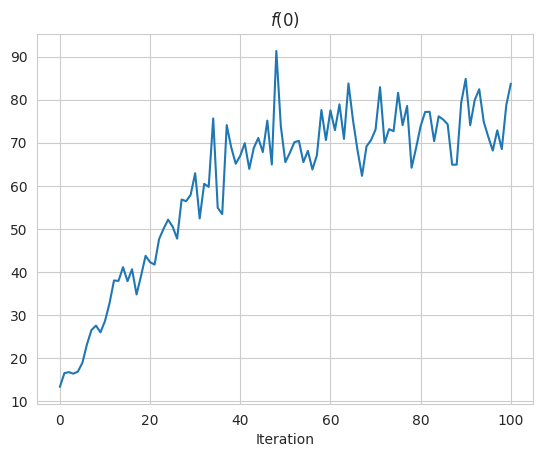
\includegraphics[width=0.9\textwidth]{images/f0.png}
        \end{figure}

        \column{0.5\textwidth}
        \begin{figure}
            \centering
            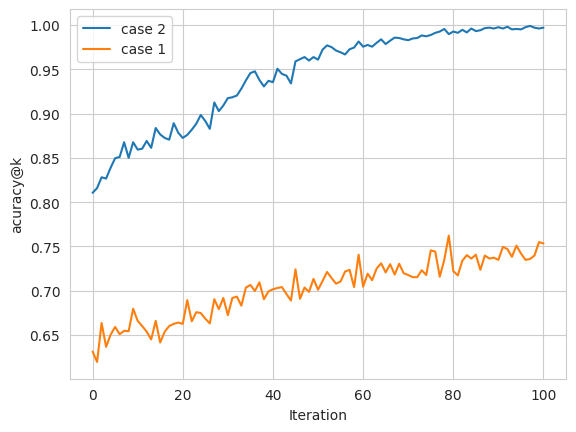
\includegraphics[width=0.9\textwidth]{images/accuracyk.png}
        \end{figure}

    \end{columns}

    \begin{figure}
        \centering
        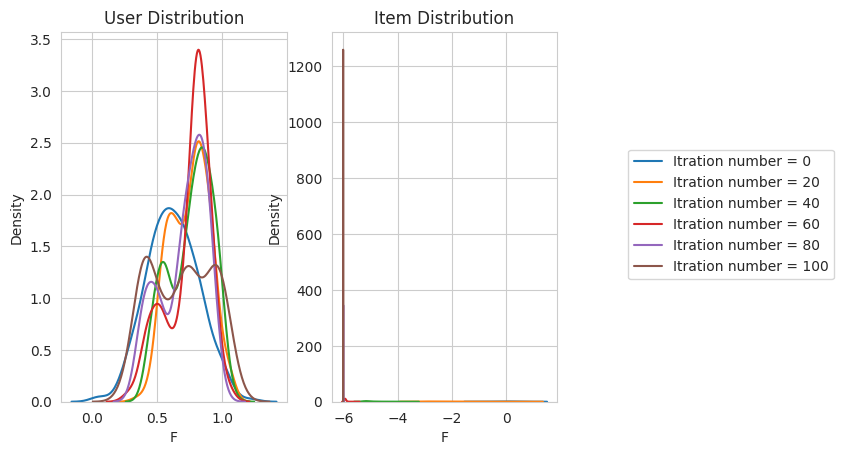
\includegraphics[width=0.8\textwidth]{images/distrChang2.png}
    \end{figure}
    
\end{frame}

%----------------------------------------------------------------------------------------------------------



\begin{frame}

    Вырождения на распределениях нет
    \begin{figure}
        \centering
        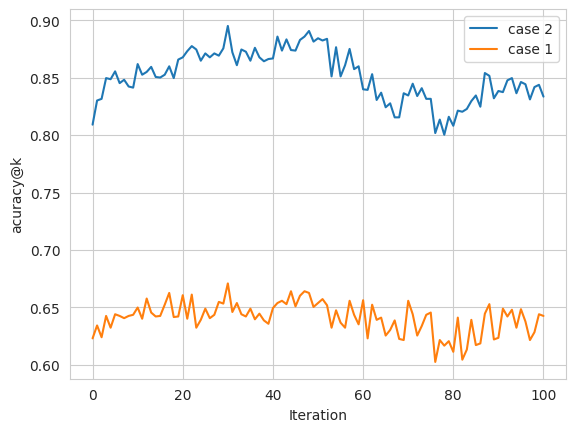
\includegraphics[width=0.5\textwidth]{images/noDegacc.png}
    \end{figure}

    \begin{figure}
        \centering
        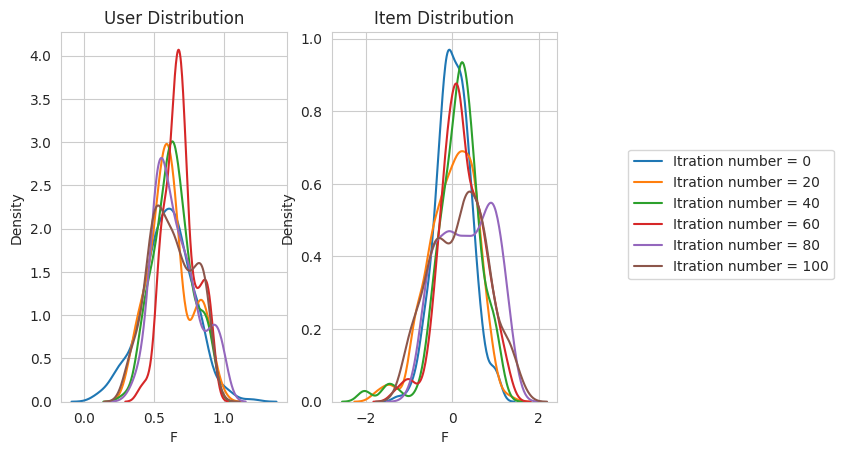
\includegraphics[width=0.8\textwidth]{images/noDeg.png}
    \end{figure}


    
\end{frame}


%----------------------------------------------------------------------------------------------------------


\begin{frame}{Заключение}
\begin{itemize}
    \item Рассмотрены различные подходы к оцениванию реальной функции полезности и предложены гипотезы о вырождениях распределений в зависимости от этих функций.
    \item Проведен вычислительный эксперимент на синтетических данных.
\end{itemize}

Планы:\\
Доказать гипотезы из теории.\\
Поставить большее количество экспериментов с различными алгоритмами.

    
\end{frame}

%----------------------------------------------------------------------------------------------------------

\end{document} 